\documentclass{beamer}
\usepackage{siunitx}
\usepackage{tfrupee}
\renewcommand{\vec}[1]{\mathbf{#1}}
\mode<presentation>
\usepackage{amsmath}
\usepackage{amssymb}
%\usepackage{advdate}
\usepackage{adjustbox}
%\usepackage{subcaption}
\usepackage{multicol}
\usepackage{mathtools}
\usepackage{listings}
\usepackage{url}
\usetheme{Boadilla}
\usecolortheme{lily}
\setbeamertemplate{footline}
{
  \leavevmode%
  \hbox{%
  \begin{beamercolorbox}[wd=\paperwidth,ht=2.25ex,dp=1ex,right]{author in head/foot}%
    \insertframenumber{} / \inserttotalframenumber\hspace*{2ex} 
  \end{beamercolorbox}}%
  \vskip0pt%
}
\setbeamertemplate{navigation symbols}{}
\providecommand{\nCr}[2]{\,^{#1}C_{#2}} % nCr
\providecommand{\nPr}[2]{\,^{#1}P_{#2}} % nPr
\providecommand{\mbf}{\mathbf}
\providecommand{\pr}[1]{\ensuremath{\Pr\left(#1\right)}}
\providecommand{\qfunc}[1]{\ensuremath{Q\left(#1\right)}}
\providecommand{\sbrak}[1]{\ensuremath{{}\left[#1\right]}}
\providecommand{\lsbrak}[1]{\ensuremath{{}\left[#1\right.}}
\providecommand{\rsbrak}[1]{\ensuremath{{}\left.#1\right]}}
\providecommand{\brak}[1]{\ensuremath{\left(#1\right)}}
\providecommand{\lbrak}[1]{\ensuremath{\left(#1\right.}}
\providecommand{\rbrak}[1]{\ensuremath{\left.#1\right)}}
\providecommand{\cbrak}[1]{\ensuremath{\left\{#1\right\}}}
\providecommand{\lcbrak}[1]{\ensuremath{\left\{#1\right.}}
\providecommand{\rcbrak}[1]{\ensuremath{\left.#1\right\}}}
\theoremstyle{remark}
\newtheorem{rem}{Remark}
\newcommand{\sgn}{\mathop{\mathrm{sgn}}}
\usepackage{enumitem}
\providecommand{\res}[1]{\Res\displaylimits_{#1}} 
\providecommand{\norm}[1]{\left\lVert#1\right\rVert}
\providecommand{\mtx}[1]{\mathbf{#1}}
\providecommand{\abs}[1]{\left\vert#1\right\vert}
\providecommand{\fourier}{\overset{\mathcal{F}}{ \rightleftharpoons}}
%\providecommand{\hilbert}{\overset{\mathcal{H}}{ \rightleftharpoons}}
\providecommand{\system}{\overset{\mathcal{H}}{ \longleftrightarrow}}
	%\newcommand{\solution}[2]{\textbf{Solution:}{#1}}
%\newcommand{\solution}{\noindent \textbf{Solution: }}align
\providecommand{\dec}[2]{\ensuremath{\overset{#1}{\underset{#2}{\gtrless}}}}
\newcommand{\myvec}[1]{\ensuremath{\begin{pmatrix}#1\end{pmatrix}}}

\title{Matrices in Geometry - 12.259}
\author{EE25BTECH11037  Divyansh}
\date{Sept, 2025}

\begin{document}

\maketitle


\section{Problem}
\begin{frame}
\frametitle{Problem Statement}
Consider the system of equations
\begin{align*}
    \myvec{5 & 2 & 1 \\ -2 & 5 & 2 \\ -1 & 2 & 8}\myvec{x_1 \\ x_2\\ x_3}=\myvec{13 \\ -22 \\ 14}
\end{align*}
With an initial guess of the solution $\myvec{x_1 & x_2& x_3}^{\top} = \myvec{1 & 1& 1}^{\top}$ , the approximate value of the solution $\myvec{x_1 & x_2& x_3}^{\top}$ after one iteration of the Gauss-Seidel method is
\begin{enumerate}[label=(\alph*)]
    \item $\myvec{2 & -4.4& 1.625}^{\top}$
    \item $\myvec{2 & 4.4& 1.625}^{\top}$
    \item $\myvec{2 & -4& -3}^{\top}$
    \item $\myvec{2 & -4& 3}^{\top}$
\end{enumerate}
\end{frame}

\section{Solution}
\begin{frame}{Solution}
Let the initial guess of the solution be 
\begin{align}
    \myvec{x_1 \\ x_2\\ x_3}=\myvec{1 \\1 \\1}
\end{align}
Isolating each variable from the given equations 
\begin{align}
    x_1=\dfrac{13-2x_2-x_3}{5} \ , \ 
    x_2=\dfrac{-22+2x_1-2x_3}{5} \ , \ 
    x_3=\dfrac{14+x_1-2x_2}{8}
\end{align}
Substituting $x_2=1, x_3=1$ in the first equation
\begin{align}
    x_1=\dfrac{13-2-1}{5} = \dfrac{10}{5} =2
\end{align}
\end{frame}

\begin{frame}{Solution}
Substituting $x_1=2 , x_3=1$ in the second equation
\begin{align}
    x_2=\dfrac{-22+4 -2}{5} = \dfrac{-20}{5} =-4
\end{align}
Substituting $x_1=2, x_2 = -4$
\begin{align}
    x_3=\dfrac{14+2+8}{8}=\dfrac{24}{8}=3
\end{align}
After one iteration of the Gauss-Seidel method, we get
\begin{align}
    \myvec{x_1 \\ x_2 \\ x_3 }=\myvec{2 \\ -4 \\ 3}
\end{align}
which is option $\brak{d}$
\end{frame}
\begin{frame}{Solution}
    Plotting these points in a graph
\begin{figure}
    \centering
    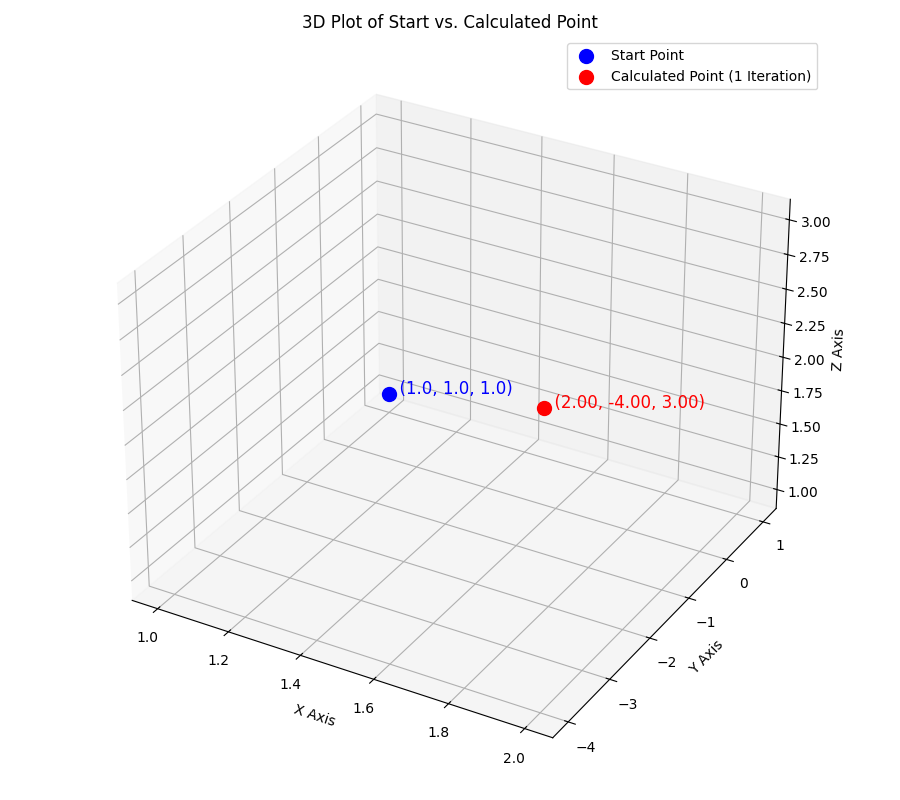
\includegraphics[width=0.5\columnwidth]{figs/1.png}
    \caption{Graph for 12.259}
    \label{fig:placeholder}
\end{figure}
\end{frame}

\end{document}
